\section{Extensions}
\label{sec:extensions}

  \subsection{Markov Model}
  \label{sec:markov_model}

  \subsection{BoW + NN}
  \label{sec:bow_nn}

  \subsection{RNN}
  \label{sec:rnn_grid_search}

    It was not clear \textit{a priori} which hyper-parameter choices were
    appropriate for the RNN. To find parameters a grid search was performed over
    the number of neurons in the recursive cell, the kind of recursive cell
    (LSTM or GRU), the dropout rate and the learning rate.

    \begin{figure}[ht]
      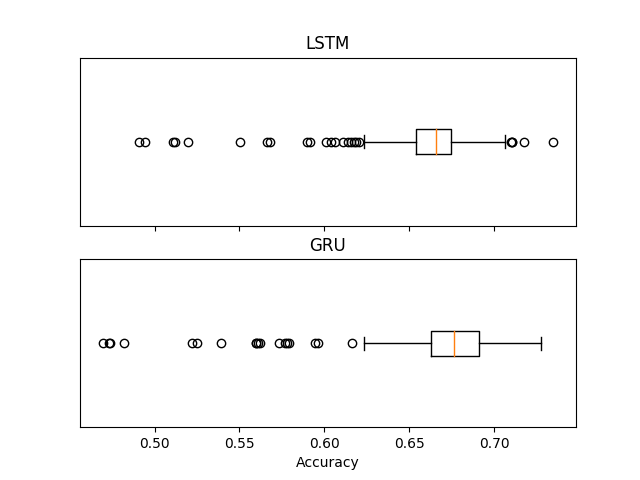
\includegraphics[width=0.45\textwidth]{Figures/lstm_gru_plot.png}
      \caption{Comparing the performance of LSTM and GRU cells over all
        parameter measurements}
      \label{fig:lstm_gru}
    \end{figure}

    Figure \ref{fig:lstm_gru} compares the performance of LSTM and GRU cells
    over all measurements. The GRU cell achieved a higher
    median, lower and upper quartile accuracy than the LSTM cell. However, including
    outliers, the GRU cell was less consistent: achieving the lowest accuracy
    single result. The highest accuracy was an LSTM cell but this was only by a
    small margin.

    \begin{figure}[ht]
      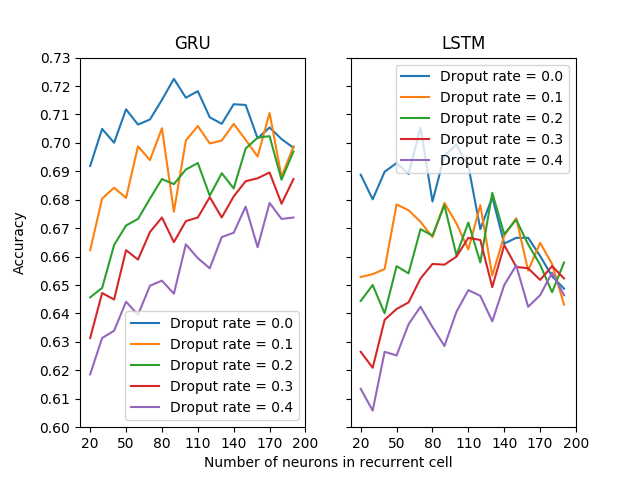
\includegraphics[width=0.45\textwidth]{Figures/n_neurons_plot-0-0001.png}
      \caption{Using a learning rate of 0.0001: the relationship between the number of neurons in the recurrent
        cell to classification accuracy for GRU and LSTM at each dropout rate.}
      \label{fig:learn_rate_0.0001}
    \end{figure}

    Figure \ref{fig:learn_rate_0.0001} shows the results for training using a
    learning rate of 0.0001. At this learning rate the GRU saw slight improvements in
    accuracy with an increasing number of neurons up to 100, after which
    accuracy declined. This decline was likely due to minor overfitting of the
    training set. However, even the lowest dropout rates only approached
    performance on par with no dropout for the largest numbers of neurons
    tested. For most of the data, there was a clear accuracy reduction from an
    increase in the dropout rate.

    The LSTM cell performed much less well than GRU at this learning rate, with
    classification accuracy quickly declining for numbers of neurons higher than
    110. The dropout rate was similarly detrimental as for the GRU at
    small numbers of neurons. As performance degraded at higher numbers of
    neurons, moderate dropout rates (up to 0.2) out-performed the network without
    dropout. This suggests more severe overfitting than for the GRU cell,
    perhaps because LSTM is a more complex construction. 

    \begin{figure}[ht]
      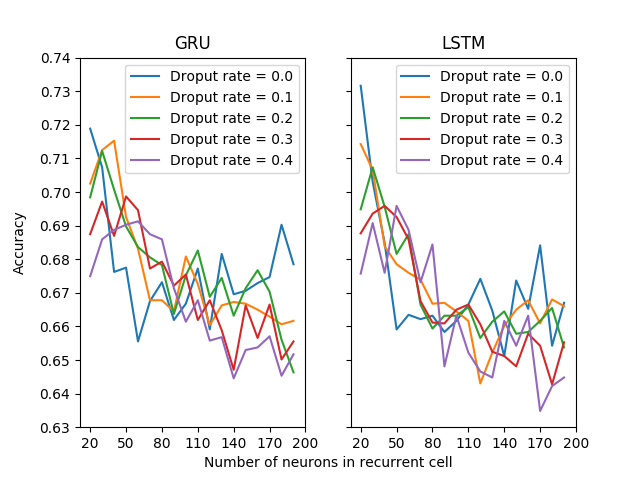
\includegraphics[width=0.45\textwidth]{Figures/n_neurons_plot-0-001.png}
      \caption{Using a learning rate of 0.001: the relationship between the number of neurons in the recurrent
        cell to classification accuracy for GRU and LSTM at each dropout rate.}
      \label{fig:learn_rate_0.001}
    \end{figure}

    Figure \ref{fig:learn_rate_0.001} shows results for a higher learning rate
    of 0.001. At this higher learning rate there was a clear performance
    degradation as the number of neurons was increased, particularly up to 100
    neurons. The results are also far more chaotic, with measurements spiking up
    and down. In further tests it was confirmed that there was a higher variance in
    the results at this learning rate compared to the previous. Results at a
    further increased learning rate of 0.01 varied so much as to be
    un-reproducible. This suggests that a learning rate of 0.001 was too high to
    capture the features of this optimisation problem, with the issue worsening
    as neurons are added: increasing the complexity of the fitness landscape.
    This higher learning rate achieved the highest accuracies in the test when
    using smaller neurons. This may indicate that the smaller 0.0001 learning rate grid
    search had not trained over sufficient epochs before stopping - giving the
    higher learning rate the upper hand in the simpler learning problems.

    Dropout rates seem to have had much less of an effect at this higher
    learning rate, however, the highest results were still mostly obtained by
    the lower dropout rates. The cell type also seemed to have much less of an
    affect. Perhaps the problems training with this higher learning rate also
    reduced overfitting.

    \subsection{Ensemble}
    \label{sec:ensemble}

    \subsection{KPCA}
    \label{sec:kpca}
  
